\chapter{Introduction}
\begin{tcolorbox}\begin{center}
Un sistema \'e un entit\'a artificiale o fisica che evolve nel tempo. Spesso conviene definire un sistema come la relazione fra segnali in input e in output.
\end{center}\end{tcolorbox}
Un \textbf{segnale} \'e una funzione che descrive il sistema nel suo evolvere di quantit\'a col passare del tempo. 

\begin{tcolorbox}\begin{center}
    Segnale: \textit{time$\_$space T} $\rightarrow \mathbb{U}$, dove U \'e la quantit\'a in questione. \\
\end{center}\end{tcolorbox}

Denoto una classe di segnali come:
$\mathcal{U}=\{u(\cdot):\mathcal{T} \rightarrow \mathbb{U}\}$

\section{Time space}
Per il time space $\mathcal{T}$ posso far riferimento a \textbf{continuous time, discrete event o discrete time}.

\subsection{Continuous Time Signals}
In continuous time descrivo quantit\'a fisiche. Un time space dev'essere totalmente ordinato, metrico (misurabile) e continuo (posso fare calcolo differenziale).
Tipicamente $\mathcal{T} \subset \mathbb{R}$. Lo uso se devo descrivere un circuitino ad esempio.

\subsection{Discrete Events Signals}
Nel caso di discrete events signals sono slegato dal tempo fisico, tutto quello che so \'e l'ordine degli eventi. 
Indipendentemente dal tempo fisico una sequenza in input deve dare lo stesso output. Il time space $\mathcal{T}$ dev'essere
ordinato e finito (tra due eventi devo aver un numero finito di altri eventi); pertanto uso $\mathbb{N}$. Lo uso per state transition diagrams.

\subsection{Discrete Time Signals}
Nel caso di discrete time signals ho una classe di discrete event signals con synchronous time instants. Tipicamente si sicronizzano 
gli istanti su un periodic time base. Il set dev'essere ordinato e abeliano (per poter computare somme e differenze di eventi).
Solitamente uso $\mathbb{Z}$.

Un sistema \'e formato da associazioni di sottosistemi eterogenei. 
DT (Discrete Time) systems sono ottenuti da CT (Continuous Time) systems con restrizioni temporali a quando certe quantit\'a si possono
misurare o certe variabili in input cambiano. 

Una quantit\'a fisica come il tempo viene campionata in molti periodi.
\begin{center}
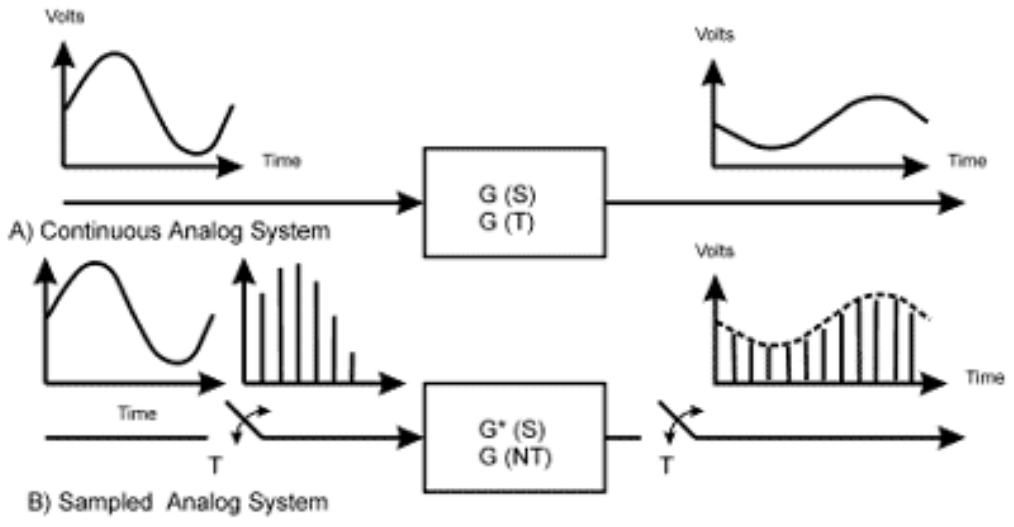
\includegraphics[scale=0.35]{Chapters/Img/c01_01.png}\\
\end{center}

Solitamente uso calligraphic letter per denotare classi di segnali $\mathcal{U} = \{ \mathcal{u} (\cdot ) : \mathcal{T} \rightarrow \mathbb{U} \}$.
\begin{center}
    Time spaces:
    \begin{tabular}{lll}
        \textbf{Continuous time (CT)} signals & \textbf{Discrete Events (DE)} signals & \textbf{Discrete Time (DT)} signals\\
        totally ordered & totally ordered & totally ordered\\
        metric & fra due eventi posso averne finiti altri & sequenze di eventi associati a istanti \\ %temporali\\
        a continuum & & gli eventi devono essere \textbf{sincroni}\\
        & & gruppi abeliani \\
    \end{tabular}
\end{center}

CT si usa per rappresentare l'evoluzione di quantit\'a fisiche pertanto solitamente uso $\mathbb{R}$.

Per discrete events la storia \'e diversa, mi interessa solo l'ordine degli input, quanto tempo passa fra un input e l'altro non cambia l'output, solitamente uso 
$\mathbb{N}$. Ho una sequenza di eventi totalmente ordinati che posso mappare su $\mathbb{N}$.

Avendo DT eventi mappati su gruppi abeliani uso $\mathbb{Z}$.

Infine ho sistemi che sono collection di sottosistemi ogniuno con potenzialmente differenti time spaces.

\chapter{Sistemi}
\begin{tcolorbox}\begin{center}
    Considero $\mathcal{U}$ la classe dei segnali di input e $\mathcal{Y}$ la classe dei segnali di output che prendono valore da $Y$. Allora posso definire 
    il \textbf{sistema} come una relazione binaria fra $\mathcal{U}$ e $\mathcal{Y} :\ S \subset \mathcal{U} \otimes \mathcal{Y}$ (una relazione binaria sar\'a un set di 
    coppie (input, output)). 
\end{center}\end{tcolorbox}

Naturalmente posso avere lo stesso output per diversi input e viceversa (se, ad esempio, cambio lo stato iniziale).\\[5pt]

Denoto:
\begin{center}
    \begin{tabular}{ll}
        $\mathcal{T}(t_0) = \{ t \in \mathcal{T}: t \geq t_0 \}$ & il sottoinsieme del time space contenente gli istanti.\\
        $\mathcal{W}^{T(t_0)} = \{ w_0(\cdot) : \forall t \geq t_0,\ t \rightarrow w_0(t) \in W$ & il set di funzioni definite su $T(t_0)$ a valori in W.\\
        $w_0|_{T(t_1)}$ & la truncation della funzione che valuto da $t_1 > t_0$.\\
    \end{tabular}
\end{center}

\begin{tcolorbox}\begin{center}
    An \textbf{abstract dynamic system} is a 3-tuple $\{ T,\ \mathcal{U} \otimes \mathcal{Y},\ \sum \}$ con \\[5pt]
    $\sum = \{ \sum (t_0) \subset \mathcal{U}^{T(t_0)} \otimes \mathcal{Y}^{T(t_0)}: t_0 \in \mathcal{T}\ AND\ CRT\ is\ satisfied\}$ \\[5pt]
    dove CRT \'e la chiusura rispetto alla truncation (i.e. $\forall\ t_1 \geq t_0$).
\end{center}\end{tcolorbox}
$(u_0,\ y_0) \in \sum (t_0) \implies (u_0|_{T(t_1)},\ y_0|_{T(t_1)}) \in \sum (t_1)$, in pratica CRT property significa che se una coppia di funzioni appartiene al sistema 
da $t_0$ in poi, esse vengono troncate da $t_1$ in poi.


